\documentclass[11pt]{article}
\usepackage[letterpaper, margin=1in]{geometry}
\usepackage{graphicx}
\graphicspath{{Images/}}
\usepackage{parskip}
\usepackage{amsmath}
\usepackage{caption}
\usepackage{hyperref}
\usepackage{xcolor}
\usepackage{setspace}
\usepackage{fancyhdr}
\usepackage{fontspec}
\usepackage{enumitem}
\setmainfont{Montserrat}

\setlength{\headheight}{40pt}
\setlength{\headsep}{20pt}


\pagestyle{fancy}
\fancyhf{}

\renewcommand{\headrulewidth}{0.5pt}
\renewcommand{\footrulewidth}{0pt}

\fancyhead[R]{
\includegraphics[height=1.5cm]{argo_space_logo.jpg}}

\fancyfoot[C]{%
  \footnotesize
  \textcolor{blue}{ARGO SPACE CORP} \textcolor{gray}{| CONFIDENTIAL \& PROPRIETARY}
}

\fancyhead[L]{\textcolor{gray}{P a g e  |  }\thepage}

\begin{document}
    \doublespacing
    \begin{titlepage}
        \centering

        
\includegraphics[width=2in]{argo-space.jpg}

        \vspace*{1.5cm}
        \Huge
        \textbf{Navigator Coupon Thermal Test Procedure}

        \vfill

        
\includegraphics[width = 1.5in]{argo_space_logo.jpg}

        \normalsize
        \textcolor{gray}{Author: Jonathan Vollrath} \\
        \textcolor{gray}{Runner: Jonathan Vollrath \& Chris Wordingham} \\
        \textcolor{gray}{Reviewer: Ben Zabback \& Chris Wordingham} \\
        \textcolor{gray}{Release Version: A} \\
        \textcolor{gray}{Written: May 8, 2025} \\
        \textcolor{gray}{Run: } \\
        \textcolor{gray}{Duration: }
    \end{titlepage}

    \section*{Release Notes}

        \begin{enumerate}[label=\Alph*.]
            \item \textbf{Initial Release}
            \begin{itemize}
                \item Outline of procedure for review by Ben
                \item Includes basic procedure for conducting thermal test of coupon
            \end{itemize}
        \end{enumerate}

    \newpage

    \section{Setup}
        \begin{enumerate}
            \item Gather thermocouple, compression fitting (blue), and tee-fitting (red) as shown below: \\
            \begin{minipage}{0.45\textwidth}
                \vspace*{1em}
                \includegraphics[width=\textwidth]{thermocouple.jpeg}
                \captionsetup{type=figure}
                \caption{Thermocouple used in testing}
            \end{minipage}
            \hfill
            \begin{minipage}{0.45\textwidth}
                \vspace*{1em}
                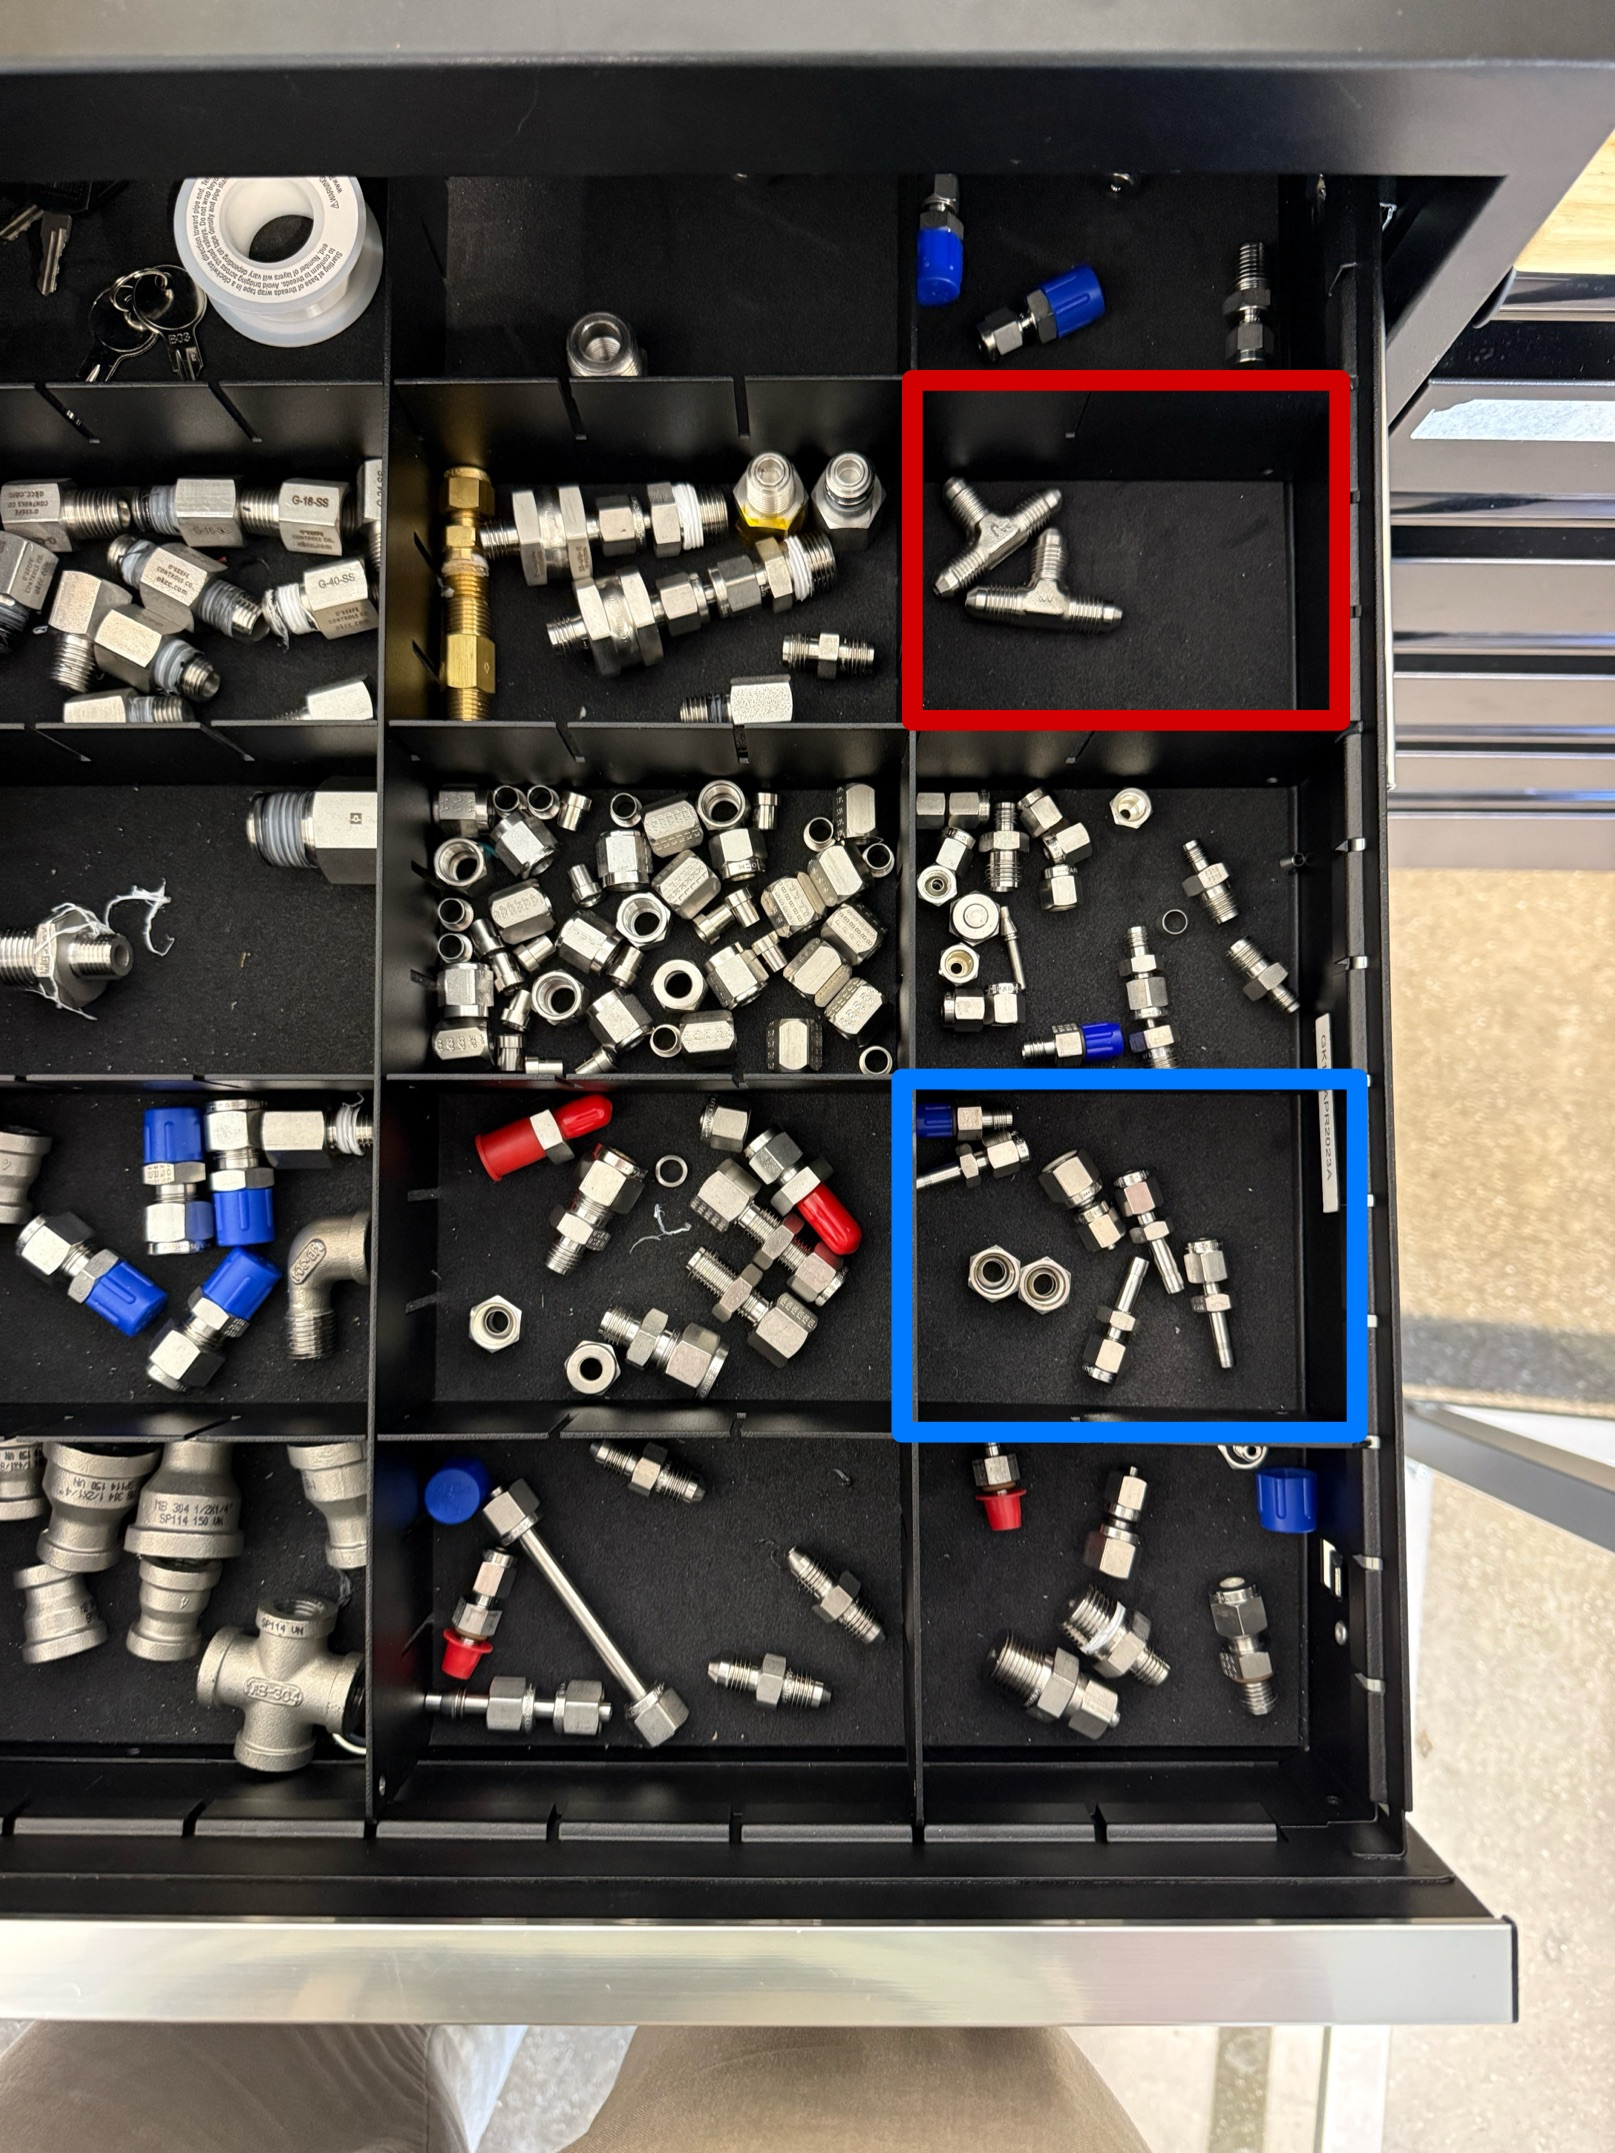
\includegraphics[width=0.75\textwidth, angle=90]{fluid_fittings.jpeg}
                \captionsetup{type=figure}
                \caption{figure}{Fittings used in testing}
            \end{minipage}
            \begin{itemize}
                \item \textbf{Note:} The compression fitting (blue) needs to be machined to accept the thermocouple (1/8 inch diameter)
                \item Notes: 
            \end{itemize}

            \item The MET nozzle coolant loop outlet is already fitted with a thermocouple, so you only need to "unplug" it and connected it to the outlet of the coupon
            \begin{itemize}
                \item Notes: 
            \end{itemize}
            \item The MET feed line does NOT have a thermocouple, and needs one
            \begin{itemize}
                \item Insert thermocouple into compression fitting, which has now been machined to accept it (all the way through)
                \item Fit compression fitting into top of tee fitting, ensuring that thermocouple is deep enough into the flow to get good reading
                \item Tighten nut on compression fitting to create water tight connection
                \item Notes: 
            \end{itemize}
            \item Connect coupon inlet to the MET feed line
            \item To set up readings from thermocouples, ask Chris (fill in later)
            \begin{itemize}
                \item Notes: 
            \end{itemize}
            \item To set up water to flow at given temp and rate, ask Chris (fill in later)
            \begin{itemize}
                \item Notes: 
            \end{itemize}
            \item Final inlet assembly should look as follows: 
            \begin{figure}[h]
                \centering
                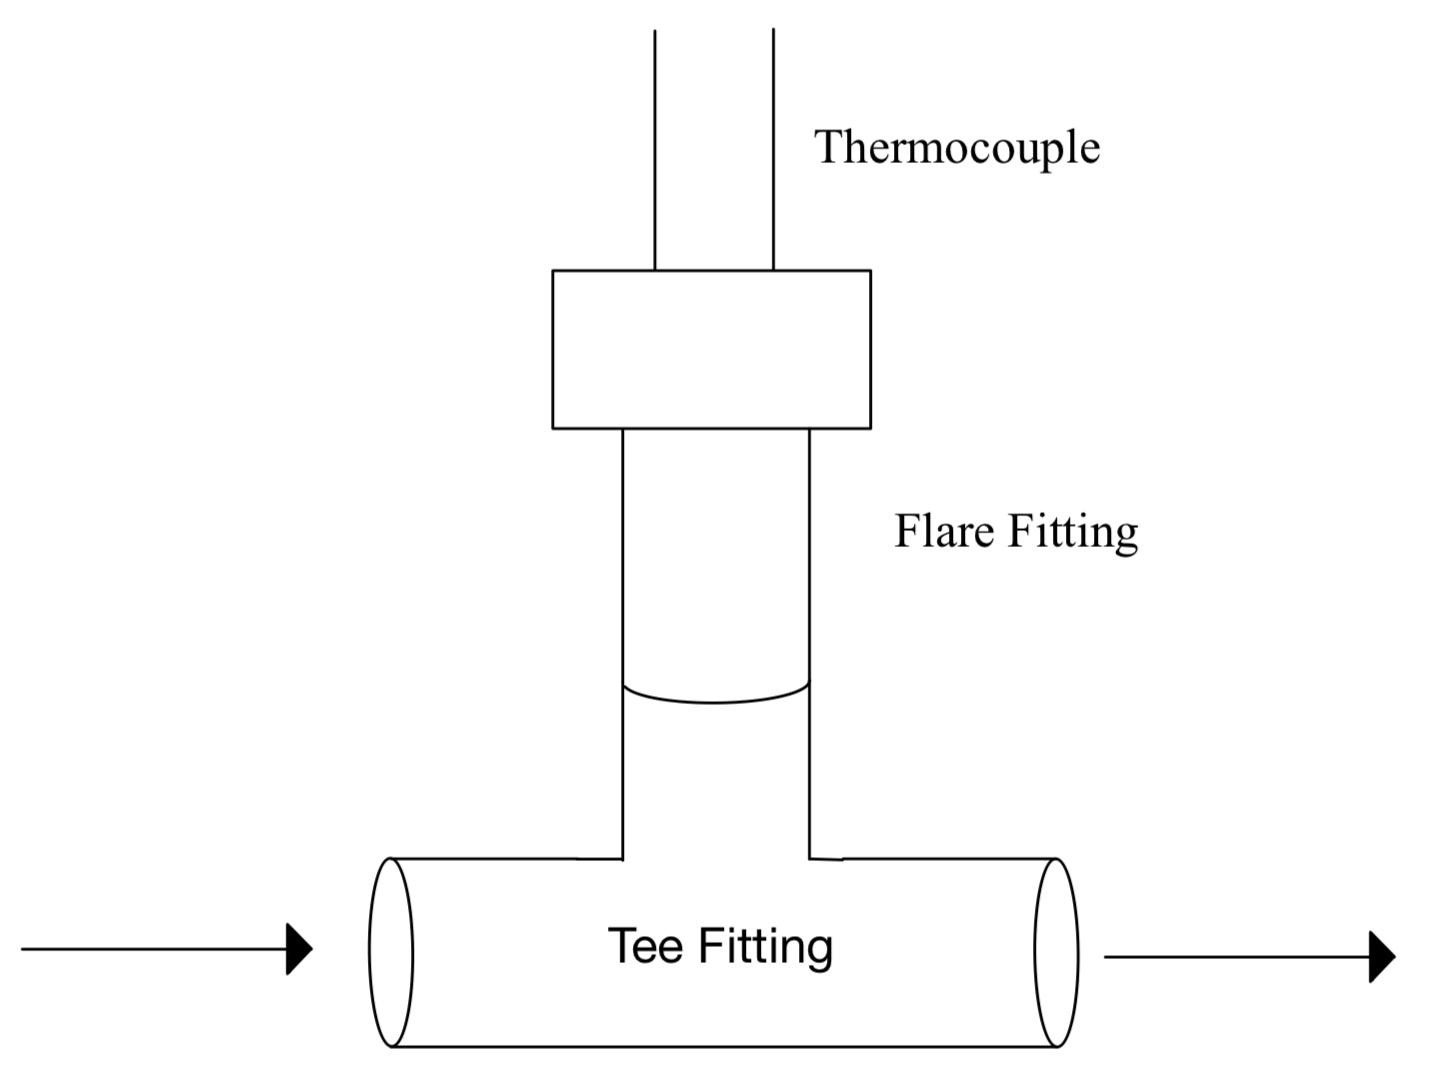
\includegraphics[width=0.5\textwidth]{fitting_assembly.jpeg}
                \caption{Inlet fitting assembly}
            \end{figure}
            \item Be ready to record vacuum chamber wall temperature during test
            \begin{itemize}
                \item Could use either thermocouple or just take a few measurements with a thermometer gun
            \end{itemize}
        \end{enumerate}

    \section{Coupon Painting}
        \begin{enumerate}
            \item 
        \end{enumerate}

    \section{Radiator Coupon Efficacy Test}
        \begin{enumerate}
            \item Pull chamber down to vacuum before taking any data
            \item Record start time
            \begin{itemize}
                \item Start Time: 
            \end{itemize}
            \item Record vacuum chamber wall temperature
            \begin{itemize}
                \item Temperature: 
                \item Time: 
            \end{itemize}
            \item Yeah, Chris knows how to run the MET flow thingy, just ask him (fill in later)
            \begin{itemize}
                \item Target flow rate of 100 $\pm$ 10 mg/s and a fluid temp of 80 $\pm$ 5 C at the coupon inlet
                \item Flow for long enough that the fluid outlet temperature has stabilized and verify the outlet temperature is at least 10 C colder than the inlet temperature. If it is not, reduce the flow rate and repeat the test until you hit at least a 10 C delta temperature
                \item One coupon outlet temperature has stabilized, hold steady flow for an additional 3 minutes
                \item Notes: 
            \end{itemize}
            \item Record vacuum chamber wall temperature
            \begin{itemize}
                \item Temperature: 
                \item Time: 
            \end{itemize}
            \item Record vacuum chamber wall temperature
            \begin{itemize}
                \item Temperature: 
                \item Time: 
            \end{itemize}
            \item Record vacuum chamber wall temperature
            \begin{itemize}
                \item Temperature: 
                \item Time: 
            \end{itemize}
            \item Record vacuum chamber wall temperature
            \begin{itemize}
                \item Temperature: 
                \item Time: 
            \end{itemize}
            \item Record endtime \& runtime
            \begin{itemize}
                \item End Time: 
                \item Runtime: 
                \item Notes: 
            \end{itemize}
        \end{enumerate}

    \newpage

    \section{Summary}

    \appendix

\end{document}
